\subsection{Diagrammi delle classi del Model}
			\subsubsection{Package Database}
			\begin{center}
				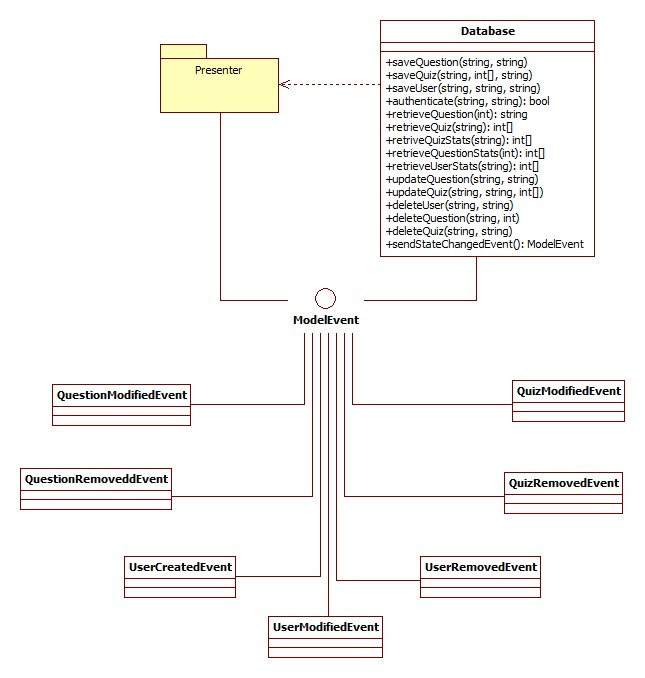
\includegraphics[scale=0.6]{../images/Database.jpg}
			\end{center}
 			\subsubsubsection{Classe Database}
 			\begin{itemize}
		    	\item\textbf{Funzione del componente:} la classe permettera' l'inserimento, la lettura, la modifica e la rimozione dei dati all'interno del database
			\item\textbf{Relazioni d'uso di altri componenti:} interagisce con il Presenter, inviando o ricevendo dati sulla base delle richieste di quest'ultimo
			\item\textbf{Attivita' svolte e dati trattati:} ogni metodo della classe consente l'inserimento, la lettura, la modifica e la rimozione di dati dal database, in seguito alla quale si possono verificare eventi per notificare al Presenter
			\end{itemize}
			\subsubsubsection{Interfaccia ModelEvent}
			\begin{itemize}
		    	\item\textbf{Funzione del componente:} l'interfaccia identifichera' dei particolari eventi che richiedono l'intervento del Presenter
			\item\textbf{Relazioni d'uso di altri componenti:} questa interfaccia verra implementata da classi che andranno a specificare un particolare tipo di evento
			\end{itemize}
			\subsubsubsection{Classe QuestionModifiedEvent}
			\begin{itemize}
		    	\item\textbf{Funzione del componente:} la classe specifica la modifica di un quesito nel database
				\item\textbf{Relazioni d'uso di altri componenti:} implementa l'interfaccia ModelEvent
				\item\textbf{Attivita' svolte e dati trattati:} segnala al Presenter il verificarsi della modifica di un quesito
			\end{itemize}
			\subsubsubsection{Classe QuestionRemovedEvent}
			\begin{itemize}
		    	\item\textbf{Funzione del componente:} la classe specifica la rimozione di un quesito nel database
				\item\textbf{Relazioni d'uso di altri componenti:} implementa l'interfaccia ModelEvent
				\item\textbf{Attivita' svolte e dati trattati:} segnala al Presenter il verificarsi della rimozione di un quesito
			\end{itemize}
			\subsubsubsection{Classe QuizModifiedEvent}
			\begin{itemize}
		    	\item\textbf{Funzione del componente:} la classe specifica la modifica di un quiz nel database
				\item\textbf{Relazioni d'uso di altri componenti:} implementa l'interfaccia ModelEvent
				\item\textbf{Attivita' svolte e dati trattati:} segnala al Presenter il verificarsi della modifica di un quiz
			\end{itemize}
			\subsubsubsection{Classe QuizRemovedEvent}
			\begin{itemize}
		    	\item\textbf{Funzione del componente:} la classe specifica la rimozione di un quiz nel database
				\item\textbf{Relazioni d'uso di altri componenti:} implementa l'interfaccia ModelEvent
				\item\textbf{Attivita' svolte e dati trattati:} segnala al Presenter il verificarsi della rimozione di un quiz
			\end{itemize}
			\subsubsubsection{Classe UserCreatedEvent}
			\begin{itemize}
		    	\item\textbf{Funzione del componente:} la classe specifica l'aggiunta di un nuovo utente nel database
				\item\textbf{Relazioni d'uso di altri componenti:} implementa l'interfaccia ModelEvent
				\item\textbf{Attivita' svolte e dati trattati:} segnala al Presenter il verificarsi dell'aggiunta di un nuovo utente
			\end{itemize}
			\subsubsubsection{Classe UserModifiedEvent}
			\begin{itemize}
		    	\item\textbf{Funzione del componente:} la classe specifica la modifica di un utente nel database
				\item\textbf{Relazioni d'uso di altri componenti:} implementa l'interfaccia ModelEvent
				\item\textbf{Attivita' svolte e dati trattati:} segnala al Presenter il verificarsi della modifica di un utente
			\end{itemize}
			\subsubsubsection{Classe UserRemovedEvent}
			\begin{itemize}
		    	\item\textbf{Funzione del componente:} la classe specifica la rimozione di un utente nel database
				\item\textbf{Relazioni d'uso di altri componenti:} implementa l'interfaccia ModelEvent
				\item\textbf{Attivita' svolte e dati trattati:} segnala al Presenter il verificarsi della rimozione di un utente
			\end{itemize}
			
			\subsubsection{Package Parser}
			\begin{center}
				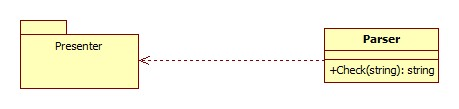
\includegraphics[scale=0.6]{../images/Parser.jpg}
			\end{center}
 			\subsubsubsection{Classe Parser}
 			\begin{itemize}
		    	\item\textbf{Funzione del componente:} controlla che il testo fornito risulti corretto secondo la sintassi QML
			\item\textbf{Attivita' svolte e dati trattati:} il Parser controlla che il testo fornito in input rispetta la sintassi QML e fornisce in caso di errore un messaggio avvertendo l'utente di dove si trova l'errore e la tipologia
			\end{itemize}
			
			\subsubsection{Package Statistiche}
			\begin{center}
				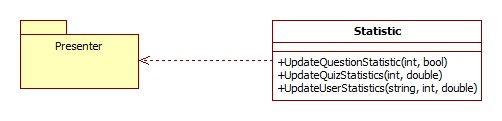
\includegraphics[scale=0.6]{../images/Statistics.jpg}
			\end{center}
 			\subsubsubsection{Classe Statistic}
 			\begin{itemize}
		    	\item\textbf{Funzione del componente:} questa classe fornisce funzionalita' per il raccoglimento delle statistiche all'interno di Quizzipedia
			\item\textbf{Attivita' svolte e dati trattati:} la classe aggiornera' le statistiche relative ai quesiti, questionari ed utenti.
			Per i quesiti verranno indicati il numero di volte che e' stato proposto e il numero di risposte corrette.
			Per i questionari verranno indicati le valutazioni medie ottenute dagli utenti e il numero di volte che e' stato proposto.
			Per gli utenti verranno indicati la valutazione migliore e la media dei tentativi eseguiti su singolo quiz
			\end{itemize}